\tikzstyle{input_neuron}=[circle,draw=red!50,fill=red!10,thick,minimum size=6mm]
\tikzstyle{hidden_neuron}=[circle,draw=blue!50,fill=cyan!10,thick,minimum size=6mm]
\tikzstyle{output_neuron}=[circle,draw=green!50,fill=green!10,thick,minimum size=6mm]

\tikzstyle{input}=[circle,draw=black!50,fill=black!20,thick,minimum size=6mm]

\begin{center}
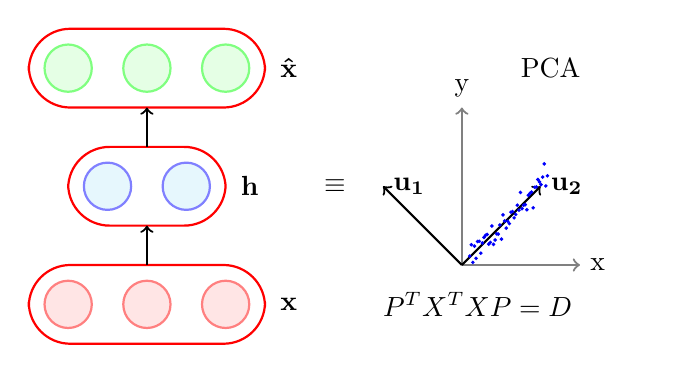
\begin{tikzpicture}


\node [input_neuron] (neuron01) at (6.5,4.5) {};
\node [input_neuron] (neuron02) at (7.5,4.5){};
\node [input_neuron] (neuron03) at (8.5,4.5) {};
%\node [input_neuron] (neuron04) at (9.5,4.5) {};
%\node [input_neuron] (neuron05) at (10.5,4.5) {};
\node [hidden_neuron] (neuron51) at (7,6) {} ;
\node [hidden_neuron] (neuron52) at (8,6)  {};
%\node [hidden_neuron] (neuron53) at (9,6)  {};
%\node [hidden_neuron] (neuron54) at (10,6)  {};

\node [output_neuron] (neuron11) at (6.5,7.5)  {};
\node [output_neuron] (neuron12) at (7.5,7.5)  {};
\node [output_neuron] (neuron13) at (8.5,7.5)  {};
%\node [output_neuron] (neuron14) at (9.5,7.5)  {};
%\node [output_neuron] (neuron15) at (10.5,7.5)  {};

\node[text width=0.01cm] at (9.2,4.5) {$\mathbf{x}$};
\node[text width=0.01cm] at (8.7,6) {$\mathbf{h}$};
\node[text width=0.01cm] at (9.2,7.5) {$\mathbf{\hat{x}}$};

\draw[red!100,thick,solid,rounded corners=15pt] (6,4) rectangle (9,5);
\draw[red!100,thick,solid,rounded corners=15pt] (6.5,5.5) rectangle (8.5,6.5);
\draw[red!100,thick,solid,rounded corners=15pt] (6,7) rectangle (9,8);


\draw[thick,->] (7.5,5) -- (7.5,5.5);

\draw[thick,->] (7.5,6.5) -- (7.5,7);


\node[text width=0.5cm] at (10,6) {$\equiv$};
  \node[text width=1.5cm] at (13,7.5) {PCA};
  \node[text width=3cm] at (12,4.5) {$P^TX^TXP=D$};
    \draw [thick, gray, ->] (11.5,5) -- (11.5,7)      % draw y-axis line
        node [above, black] {y};              % add label for y-axis
        %node [below,black]{$-y$};
    \draw [thick, gray, ->] (11.5,5) -- (13,5)      % draw x-axis line
        node [right, black] {x};  
    \draw [thick, black, ->] (11.5,5) -- (10.5,6)      % draw u1 line
        node [right, black] {$\mathbf{u_1}$}; 
    \draw [thick, black, ->] (11.5,5) -- (12.5,6)      % draw u2 line
        node [right, black] {$\mathbf{u_2}$}; 

%\if 1
\foreach \x/\y in {0.5/0.511870677093,0.520134228188/0.657474112041,0.540268456376/0.433301054831,0.560402684564/0.639402738784,0.580536912752/0.484888418032,0.60067114094/0.698401610126,0.620805369128/0.7012649978,0.640939597315/0.550258599782,0.661073825503/0.678863257247,0.681208053691/0.75063942818,0.701342281879/0.776722844493,0.721476510067/0.787974629261,0.741610738255/0.664867942136,0.761744966443/0.686496368534,0.781879194631/0.895235993285,0.802013422819/0.661601738133,0.822147651007/0.717376222072,0.842281879195/0.796219038444,0.862416107383/0.792290066926,0.88255033557/0.908555964509,0.902684563758/0.728213610997,0.922818791946/1.03682525621,0.942953020134/0.959254604949,0.963087248322/0.868395203865,0.98322147651/0.954903379431,1.0033557047/0.925500701421,1.02348993289/1.0700072327,1.04362416107/1.07910784654,1.06375838926/0.998680883498,1.08389261745/1.04215184899,1.10402684564/1.15961695354,1.12416107383/1.09641078989,1.14429530201/1.32135817413,1.1644295302/1.11554678055,1.18456375839/1.15881333579,1.20469798658/1.16650720076,1.22483221477/1.10170000196,1.24496644295/1.2856802819,1.26510067114/1.31032588214,1.28523489933/1.32664087434,1.30536912752/1.12586374789,1.3255033557/1.38744778116,1.34563758389/1.39149477354,1.36577181208/1.4858410387,1.38590604027/1.45489220706,1.40604026846/1.42066727608,1.42617449664/1.51638552543,1.44630872483/1.68453235672,1.46644295302/1.40404774902,1.48657718121/1.53217972768} 
                {
                \node at (11.1+\x,4.6+\y)[circle,draw=blue,fill=black,inner sep=0pt,minimum size=0.3mm]{};
                }
%\fi 
\end{tikzpicture} 
\end{center}
